
\section{cuGAL}
We now describe the different stages of the cuGAL algorithm in detail.

\subsection{Sinkhorn-Knopp}
As mentioned in Section \ref{float_speed}, modern GPUs are optimised for 32-bit floats. This poses a challenge for Sinkhorn-Knopp, which is prone to overflows. Using 32-bit floats results in overflows at values exceeding $3.4 \times 10^{38}$ \citep{ieeefloat}. In the Sinkhorn-Knopp algorithm, we perform computations of the form $e^{-x}$. This means that if $A$ contains entries below approximately $-88.72$ an overflow will occur, as $3.4 \times 10^{38} \lesssim e^{-88.72}$. A solution to this problem is doing all calculations in the log-domain. Performing Sinkhorn-Knopp iterations in the log domain is not a new technique, and has before been used to avoid issues arising from numerical instability \citep{chizat2017sinkhornlog}. %although to the best of our knowledge, no specific publication first introduced this adaptation of the Sinkhorn-Knopp algorithm.

\subsubsection{Log-Variant}
\begin{algorithm}[H]
\caption{Sinkhorn-Knopp-log}\label{alg:sinkhorn_log}
\textbf{Input:} $A \in \mathds{R}^{n \times n}, a, b \in \mathds{R}^{n}, \epsilon \in \mathds{R}$
\begin{algorithmic}[1]
\State $K \gets -A / \epsilon$
\State $a, b \gets \log(a), \log(b)$
\State $u \gets \text{initial guess, see Section \ref{warm-start}}$
\For{$i \gets 1, .., \text{it}$}
    \State $v \gets b - \texttt{logsumexp}(K + \begin{bmatrix} u & .. & u \end{bmatrix})$ \Comment{For each row}
    \State $u \gets a - \texttt{logsumexp}(K^T + \begin{bmatrix} v & .. & v \end{bmatrix})$ \Comment{For each row}
    \If {stop condition met}
        \State \textbf{break}
    \EndIf
\EndFor
\State \Return $\exp(K + \begin{bmatrix} u & .. & u \end{bmatrix} + \begin{bmatrix} v & .. & v \end{bmatrix}^T)$
\end{algorithmic}
\end{algorithm}

\texttt{logsumexp} is defined as:
\begin{equation}
    \begin{split}
        \texttt{logsumexp}(x) = \log(\sum_{i = 1}^n e^{x_i}) = \log(\sum_{i = 1}^n e^a e^{x_i - a}) = \log(e^a \sum_{i = 1}^ne^{x_i - a}) = a +\log(\sum_{i = 1}^ne^{x_i - a})
    \end{split}
\end{equation}

$a$ can be defined as $a = \max(x)$, which ensures that the largest exponent calculated is $\exp(0) = 1$. \\

We provide an efficient CUDA implementation of Sinkhorn-Knopp-log using \textit{kernel fusion}. We specifically avoid writing the results of $K + \begin{bmatrix} u & .. & u \end{bmatrix}$ and $K^T + \begin{bmatrix} v & .. & v \end{bmatrix}$ to memory by performing each scaling operation in a single fused kernel.

We assign a thread block in CUDA to calculate \texttt{logsumexp} across the rows of $A$ in parallel. We realise that because peak memory usage is used calculating the gradient, we can store the transpose of $A$ in memory without increasing memory requirements. This allows us to only have blocks collaborate across rows, which leads to favourable memory access patterns as we store all matrices as row-major layout. For further details, see CUDA source code in Appendix \ref{sinkhorn_log_impl}.

\subsubsection{Mix-Variant}
For large graphs, Sinkhorn-Knopp-log can be slow as a result of performing the $O(n^2)$ $\exp$ operations each iteration requires, which is significantly more ALU (Arithmetic Logical Unit) intensive compared to operations such as multiplication and addition.

We provide a simple, and as far as we are aware, novel solution that avoids overflows for 32-bit integers with precision close to Sinkhorn-Knopp-log in many cases. We call this method Sinkhorn-Knopp-mix, as it performs a single row scaling in the log domain before continuing using the classic Sinkhorn-Knopp algorithm.

\begin{algorithm}[H]
\caption{Sinkhorn-Knopp-mix}\label{alg:sinkhorn_mix}
\textbf{Input:} $A \in \mathds{R}^{n \times n}, a, b \in \mathds{R}^{n}, \epsilon \in \mathds{R}$
\begin{algorithmic}[1]
\State $K \gets -A / \epsilon$
\State $v \gets \log(b) - \texttt{logsumexp}(K)$
\State $K \gets \exp(K + \begin{bmatrix} v & .. & v \end{bmatrix}^T)$
\State $u \gets \text{initial guess, see Section \ref{warm-start}}$
\For{$i \gets 1, .., \text{it}$}
    \State $v \gets \frac{b}{uK}$
    \State $u \gets \frac{a}{Kv}$
    \If {stop condition met}
        \State \textbf{break}
    \EndIf
\EndFor

\State \Return $\text{diag}(u)K\text{diag}(v)$

\end{algorithmic}
\end{algorithm}

\subsubsection{Warm Start}\label{warm-start}
Choosing an initial $u$ scaling vector is crucial for reducing the number of iterations Sinkhorn-Knopp requires to converge. The standard choice of initialising all entries with $1/n$ is sub optimal. We find that the simple choice of using the resulting $u$ from the previous Frank-Wolfe iteration works very well in most cases, especially when the amount of noise is low.
\pgfplotstableread[col sep=comma]{data/sums.csv}\cache
\begin{figure}[H]
    \centering
    \begin{tikzpicture}
        \begin{axis}[
            width=\linewidth*0.5,
            xlabel={Noise},
            ylabel={Time (s)},
            xtick=data,
            xticklabels = {0.00, 0.05, 0.10, 0.15, 0.20, 0.25},
            legend pos=south west,
            legend style={at={(0.5,-0.20)}, anchor=north, legend columns=-1, font=\small},
            ymajorgrids=true,
            xmajorgrids=true,
        ]
        \addplot table[x index=\coordindex, y index=1] {\cache};
        \addplot table[x index=\coordindex, y index=2] {\cache};
        \legend{initialise with $1/n$, initialise with previous $u$}
        \end{axis}
    \end{tikzpicture}
    \caption{Running time of \textsc{cuGAL} with Sinkhorn-Knopp-mix \ref{alg:sinkhorn_mix} (MIX) with and without the warm start described in Section \ref{warm-start} on bio-dmela with varying levels of noise.}
    \label{fig:SK_accu}
\end{figure}


\subsubsection{Stop Condition}
The most traditional choice of stopping condition is checking whether the sums of the columns and rows of $\text{diag}(u)K\text{diag}(v)$ has converged close to $a$ and $b$. Instead, we choose to stop when the scaling vectors $u$ and $v$ have converged to a stable point. We take inspiration from \cite{li2023importance}, where the absolute difference between the scaling vectors from the previous iteration is considered. We specifically use the following condition for some vector $a$ and threshold $\delta$:
\begin{equation}
    \frac{\max(|a^{(i)} - a^{(i - 1)}|)}{\max(\max(|a|), \max(|a^{(i - 1)}|))} < \delta
\end{equation}

We use a relative difference to better adapt to cost matrices with high entries. The difference compared to the more traditional choice of checking for convergence mainly has to do with numeric stability. We observe that using 32-bit floats can halt the rate of convergence in certain numerically tricky situations. Checking only $u$ and $v$ also has the advantage of being faster, making it less computationally expensive to check for convergence.

If $\delta$ is chosen to be too high, Sinkhorn-Knopp will exit before properly converging which will cause a drop in accuracy. On the other hand, choosing a $\delta$ too small, will result in many redundant iterations. We find that determining a general set point where the threshold begins to hurt accuracy is challenging. Testing certain experiments with varying thresholds, we observe very significant drops in accuracy for higher thresholds, while for others, we observe almost no drop to accuracy. This can be the case on similar datasets, using similar settings. Anecdotally, we observe that the mix-variant responds worse to higher values than the log-variant. In Figure \ref{fig:SK_accu}, we see an example of this inconsistency, where even for very high $\delta$s, accuracy seems high, until it suddenly drops. 

\pgfplotstableread[col sep=comma]{data/sink_thres_bd_accu.csv}\sinkthresbdaccu
\begin{figure}[H]
    \centering
    %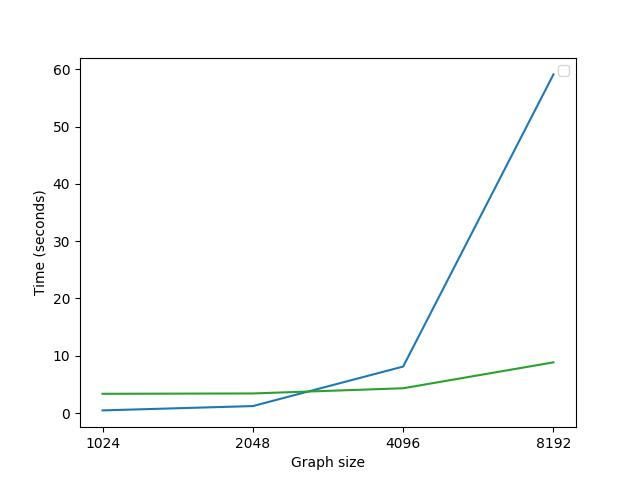
\includegraphics[width=\textwidth]{figures/sparse_vs_normal_gradient_time.jpg}
    \begin{tikzpicture}
        \begin{axis}[
            width=\linewidth*0.5,
            xlabel={Noise},
            ylabel={Accuraccy},
            x dir=reverse,
            legend pos=south west,
            xtick=data,
            xticklabels={$0.0$, $0.1$, $0.2$, $0.3$, $0.4$, $0.5$},
            %yticklabel={\pgfmathprintnumber[fixed,precision=2]{\tick}},
            legend style={at={(0.5,-0.20)}, anchor=north, legend columns=4, font=\small},
            ymajorgrids=true,
            xmajorgrids=true,
        ]
        \pgfplotsforeachungrouped \i in {0, 1, 2, 3, 4, 5, 6, 7} {
            \addplot table[x index=0, y expr=\thisrowno{\i}] 
            {\sinkthresbdaccu};
            }
        \legend{\textsc{LOG} $\delta = 0.1$, \textsc{LOG} $\delta = 0.3$, \textsc{LOG} $\delta = 0.5$, \textsc{LOG} $\delta = 1.0$,\textsc{MIX} $\delta = 0.1$, \textsc{MIX} $\delta = 0.3$, \textsc{MIX} $\delta = 0.5$, \textsc{MIX} $\delta = 1.0$}
        \end{axis}
    \end{tikzpicture}
    \caption{Accuracy of different levels of Sinhorn-Knopp threshold using \textsc{cuGAL} with Sinkhorn-Knopp-mix \ref{alg:sinkhorn_mix} (MIX) and \textsc{cuGAL} with Sinkhorn-Knopp-log \ref{alg:sinkhorn_log} (LOG) running on bio-dmela with varying levels of noise.}
    \label{fig:SK_accu}
\end{figure}

We make use of the same regularisation parameter $\epsilon$ and max iteration count $it$ as the implementation given by \cite{fugal2024}, namely $\epsilon = 1$ and $it = 300$.

\subsection{Gradient}
\subsubsection{Sparse Adjacency Matrices}
Working directly with dense adjacency matrices can be memory intensive as each instance requires $O(n^2)$ memory. To exploit the usual sparsity of adjacency matrices, we represent $A$ and $B$ using sparse matrix representations.\\

We use the popular representation CSR (Compressed Sparse Row) \citep{tinney1967csr}. For some $M \in \mathds{R}^{n \times n}$, the CSR representation consists of three vectors: $(C, R, V)$. $|C| = |V| = nnz(M)$, $|R| = n$ where $nnz(M)$ is the number non-zero entries in $M$. $C$ contains column indices of all non-zero entries in each row, starting from row 0. $R$ defines offset into $C$ where each row begins. $V$ contains the value of each non-zero element in the matrix. Because we only represent adjacency matrices of the form $\{0, 1\}^{n \times n}$, we can omit the $V$ vector.\\

CSR representation is especially well suited for matrix multiplications of the form $S \cdot D$, where $S$ is represented using CSR and $D$ is dense.

If we rewrite:
\begin{equation}
    \begin{split}
    \nabla f(P) &= -APB^T - A^TPB + \mu \cdot D\\
    &= (B^T(-A^TP)^T)^T - (B(AP)^T)^T + \mu \cdot D
    \end{split}
\end{equation}

the gradient can be calculated using only matrix multiplication of the form $S \cdot D$. This requires $A^T$ and $B^T$ to either be recalculated in each iteration or stored explicitly. If the graphs are undirected, we can exploit the fact that $A = A^T$ and $B = B^T$:
\begin{equation}
    \begin{split}
    \nabla f(x) &= (B(-AP)^T)^T - (B(AP)^T)^T + \mu \cdot D\\
    &= -2 \cdot (B (A P)^T)^T + \mu \cdot D
    \end{split}
\end{equation}

which halves the number of matrix multiplications required.

\subsubsection{Implementation}
We utilize \textit{recomputation} to avoid storing the distance matrix $D$. We instead use a custom kernel to recompute the Euclidean distances from Equation \ref{euclidean_distance_matrix} each time we compute $f(x)$. This both speeds up the computation and lowers the amount of $n \times n$ matrices required in memory by one. In addition, we use \textit{kernel-fusion} to speed up the computation of $g(x)$ by merging it with the kernel for computing $f(x)$, which avoids storing and loading intermediate results.

\begin{algorithm}[H]
\caption{sparse-calculate-gradient}\label{alg:cugal-calculate-gradient}
\textbf{Input:} $\lambda \in \mathds{R}$
\textbf{Input:} $Q \in \mathds{R}^{n \times n}$
\begin{algorithmic}[1]
\State $X \gets (B (A P)^T)^T$ \Comment{Using sparse matrix multiplication}

\For{$i, j \gets 1 \textbf{ to } \text{n}$} \Comment{In parallel}
    \State $a \gets \text{Euclidean-distance}((F_1)_{i,:}, (F_2)_{j:})$
    \State $r \gets 1 - 2Q_{i, j}$
    \State $X_{i, j} \gets -2 X_{i, j} + \mu a + \lambda r$
\EndFor

\State \Return $X$
\end{algorithmic}
\end{algorithm}

In addition, we also construct the sparse matrix representations directly from edge lists of the form $E \in (\mathds{Z_+}, \mathds{Z_+})^m$ on the GPU.

\begin{algorithm}[H]
\caption{construct-adjacency}
\textbf{Input:} $E \in (\mathds{Z_+}, \mathds{Z_+})^m$
\begin{algorithmic}[1]
    \State $E \gets$ radix-sort($E$) \Comment{Sort first by row then by column}
    \State $C, R \gets \vec{0}, \vec{0}$
    \For{$i \gets 1 \textbf{ to } |E| - 1$} \Comment{In parallel}
        \State $(a, \_), (b, \_) \gets E_i, E_{i + 1}$
        \State $b \gets E_{i + 1}$
        \For{$j \gets a + 1 \textbf{ to } b$}
            \State $R_j \gets i + 1$
        \EndFor
    \EndFor
    \For {$i \gets 1 \textbf{ to } |E| - 1$} \Comment{In parallel}
        \State $(\_, c) \gets E_i$
        \State $C_i \gets c$
    \EndFor
    \State \Return $C, R$
\end{algorithmic}
\end{algorithm}

\subsubsection{Performance}
\pgfplotstableread[col sep=comma]{data/memory_usage.csv}\mem

\begin{figure}[H]
    \centering
\begin{tikzpicture}
\begin{axis}[
    ymin=0,
    xtick=data,
    xticklabels={$2^8$, $2^9$, $2^{10}$, $2^{11}$, $2^{12}$, $2^{13}$, $2^{11}$, $2^{12}$},
    legend style={at={(0.285, 1)}, anchor=north, legend columns=1},
    bar width=12pt,
    width=\textwidth*0.5,
    xlabel={Graph size},
    ylabel={Peak memory usage in bytes},
    ymajorgrids=true,
    xmajorgrids=true,
]
\addplot table[x expr=\coordindex, y index=0] {\mem};
\addplot table[x expr=\coordindex, y index=1] {\mem};
\addplot table[x expr=\coordindex, y index=2] {\mem};
\legend{\textsc{Fugal}, \textsc{cuGAL} dense, \textsc{cuGAL} sparse}
\end{axis}
\end{tikzpicture}
    \caption{Scaling of peak memory usage of \textsc{Fugal} and \textsc{cuGAL} on NW graphs with parameters $k=7, p=0.1$ and no noise.}
    \label{fig:fugal-scaling}
\end{figure}

\begin{figure}[H]
    \centering
    %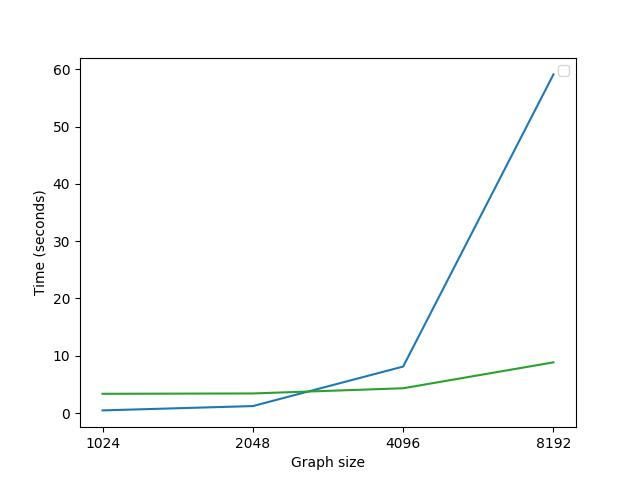
\includegraphics[width=\textwidth]{figures/sparse_vs_normal_gradient_time.jpg}
    \begin{tikzpicture}
        \begin{axis}[
            xlabel={Graph size},
            ylabel={Time (s)},
            ymajorgrids=true,
            xmajorgrids=true,
            xtick={1024, 2048, 4096, 8092},
            xticklabels={$2^{11}$, $2^{12}$, $2^{13}$, $2^{14}$},
            legend style={at={(0.7, 1)}, font=\small},
            width=\textwidth*0.5,
        ]
        \addplot table {data/dense_gradient_NSW_k10_p05.dat};
        \addplot table {data/sparse_gradient_NSW_k10_p05.dat};
        \legend{Dense (Algorithm \ref{alg:calculate-gradient}), Sparse (Algorithm \ref{alg:cugal-calculate-gradient})}
        \end{axis}
    \end{tikzpicture}
    \caption{Time spent calculating gradient for NW graphs with parameters $k=10$, $p=0.5$.}
    \label{fig:sparse_speed}
\end{figure}

Figure \ref{fig:sparse_speed} portrays the performance of using the sparse matrix multiplication for the calculating the gradient for Newmann-Watts graphs with node degree $k = 10$ and rewrite probability $p = 0.5$. While using dense adjacency matrices show better performance for smaller graphs, we observe better scaling of sparse matrix multiplication for larger graphs.

From Figure \ref{fig:fugal-scaling} we observe a significant decrease in memory from using sparse adjacency matrices. Along with more inline operations and using 32-bit floats instead of 64-bit floats, we also observe significantly lower memory usage compared to \textsc{Fugal}.

\subsection{Feature Extraction}
Feature extraction has a computational cost of $O(nM^2)$ where $M$ is the maximum degree of any vertex \citep{fugal2024}. As observed, this takes up a minor part of the overall runtime of \textsc{Fugal} (Figure \ref{fig:fugal-scaling}). However, we observe that as we optimise the rest of the algorithm, feature extraction can take up a significant part of runtime for large graphs. We therefore implement an optimised GPU implementation of feature extraction.\\

To avoid the memory cost of dense adjacency matrices, we work directly with CSR-compressed representations. 

\begin{algorithm}[H]
\caption{vertex-features}\label{alg:cugal-vertex-features}
\textbf{Input:} $(C, R, V)$ \Comment{CSR compressed matrix.}
\begin{algorithmic}[1]
\State $D \gets \vec{0}, C \gets \vec{0}$ \Comment{Vertex degrees and clustering coefficients}
\For{$i \gets 1, .., \text{n}$} \Comment{In parallel}
    \For{$j \gets R_i \textbf{ to } R_{i + 1}$} \Comment{For every neighbor}
        \State $A \gets \{ C_k | k \in R_i, .., R_{i + 1} \}$
        \State $B \gets \{ C_k | k \in R_j, .., R_{j + 1} \}$
        \State $C_i \gets C_i + |A \cap B|$
    \EndFor
    \State $D_i \gets R_{i + 1} - R_i$
\EndFor
\State \Return $D$, $C$
\end{algorithmic}
\end{algorithm}

Because the column indices of $C$ are sorted, the intersection size can be found in linear time without additional memory. Finding the average features of neighbours is done in a similar fashion.\\

We acknowledge that even more optimised implementations are possible, as our implementation can experience occupancy issues for graphs where the degree of nodes varies a lot across nodes. We restrain from further optimisations, as our implementation sufficiently improves the performance of feature extraction to make it an insignificant part of the overall runtime.

\subsection{Frank-Wolfe}
\textsc{FUGAL} performs a fixed amount of Frank-Wolfe iterations. However, we observe that the number of iterations required to converge varies depending on the graph and noise level. We define a threshold $\gamma$ on the change to $Q$ which allows us to stop early in certain cases. The threshold must not be too large, as this has two adverse effects. Firstly, the Hungarian algorithm requires more iterations to find the optimal assignment, and secondly, if the resulting difference is too large, some assignments might differ and decrease accuracy. To find a fitting threshold, we run experiments on real datasets with varying levels of synthetic noise.\\

\pgfplotstableread[col sep=comma]{data/fw_thresh_bio-dmela.csv}\fwtbm
\pgfplotstableread[col sep=comma]{data/fw_thres_bd_times.csv}\fwtbmt
\begin{figure}[H]
    \centering
    %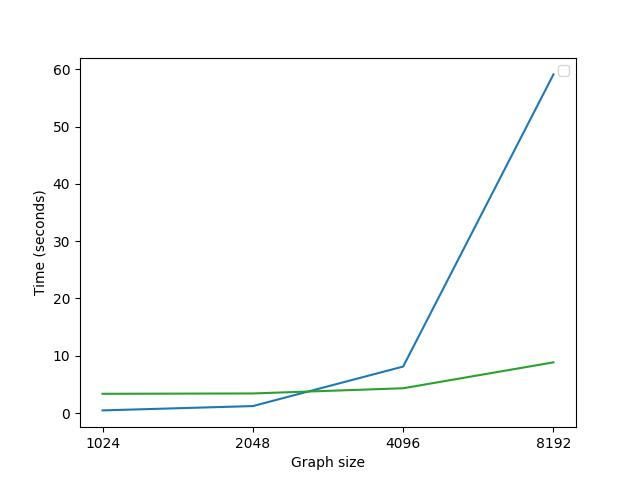
\includegraphics[width=\textwidth]{figures/sparse_vs_normal_gradient_time.jpg}
    \begin{tikzpicture}
        \begin{axis}[
            width=\linewidth*0.5,
            xlabel={Noise},
            ylabel={Accuraccy},
            x dir=reverse,
            legend pos=south west,
            xtick=data,
            xticklabels={$0.0$, $0.1$, $0.2$, $0.3$, $0.4$, $0.5$},
            %yticklabel={\pgfmathprintnumber[fixed,precision=2]{\tick}},
            legend style={at={(0.5,-0.20)}, anchor=north, legend columns=3,},
            ymajorgrids=true,
            xmajorgrids=true,
        ]
        \pgfplotsforeachungrouped \i in {1,2,3,4,5,6} {
            \addplot table[x index=0, y expr=\thisrowno{\i}] 
            {\fwtbm};
            }
        \legend{$\gamma = 0.00$, $\gamma = 0.05$, $\gamma = 0.10$, $\gamma = 0.20$, $\gamma = 0.50$, $\gamma = 1.00$}
        \end{axis}
    \end{tikzpicture}
    \caption{Accuracy of different levels of $\gamma$. \textsc{cuGAL} with Sinkhorn-Knopp-mix \ref{alg:sinkhorn_mix} on bio-dmela}
    \label{fig:FW_accu}
\end{figure}
\hfill
\begin{figure}[H]
    \begin{tikzpicture}
        \begin{semilogyaxis}[
                width=\linewidth,
                ybar stacked,
                log origin=infty,
                ylabel={Time $(s)$},
                xlabel={Noise},
                x label style={at={(0.5, -0.07)}},
                bar width=6pt,
                legend pos=south west,
                xtick=\empty,%{3.5, 10.5, 17.5, 24.5, 31.5, 38.5},
                %xticklabels={0, 5, 10, 15, 20, 25},
                %x tick label style={\empty}
                %extra x tick style={xshift=,},
                legend style={at={(0.5,-0.12)}, anchor=north, legend columns=-1},
                %yticklabel={\pgfmathprintnumber[fixed,precision=2]{\tick}},
                ymajorgrids=true,
                xmajorgrids=true,
            ]
            \pgfplotsforeachungrouped \i in {0,1,2,3} {
                    \addplot table[x expr=\coordindex, y index=\i]
                        {\fwtbmt};
                }

            %\legend{$ \displaystyle { \text{Sinkhorn-} \atop \text{Knopp} }$, $ \displaystyle { \text{Feature} \atop \text{Extraction} }$, Gradient, Hungarian};
            \legend{Sinkhorn-Knopp-mix \ref{alg:sinkhorn_mix}, Feature Extraction, Gradient \ref{alg:cugal-calculate-gradient}, Hungarian};
            \coordinate (brace1start) at (axis cs:00.5,19e-2);
            \coordinate (brace1end)   at (axis cs:07.5,19e-2);
            \coordinate (brace2end)   at (axis cs:14.5,19e-2);
            \coordinate (brace3end)   at (axis cs:21.5,19e-2);
            \coordinate (brace4end)   at (axis cs:28.5,19e-2);
            \coordinate (brace5end)   at (axis cs:35.5,19e-2);
            \coordinate (brace6end)   at (axis cs:42.5,19e-2);

        \end{semilogyaxis}
        % Adding the braces
        \draw [decorate,decoration={brace,amplitude=10pt,mirror,raise=4ex}]
        (brace1start) -- (brace1end) node[midway,yshift=-3.5em]{0};
        \draw [decorate,decoration={brace,amplitude=10pt,mirror,raise=4ex}]
        (brace1end) -- (brace2end) node[midway,yshift=-3.5em]{5};
        \draw [decorate,decoration={brace,amplitude=10pt,mirror,raise=4ex}]
        (brace2end) -- (brace3end) node[midway,yshift=-3.5em]{10};
        \draw [decorate,decoration={brace,amplitude=10pt,mirror,raise=4ex}]
        (brace3end) -- (brace4end) node[midway,yshift=-3.5em]{15};
        \draw [decorate,decoration={brace,amplitude=10pt,mirror,raise=4ex}]
        (brace4end) -- (brace5end) node[midway,yshift=-3.5em]{20};
        \draw [decorate,decoration={brace,amplitude=10pt,mirror,raise=4ex}]
        (brace5end) -- (brace6end) node[midway,yshift=-3.5em]{25};

    \end{tikzpicture}
    \caption{Speed of different levels of $\gamma$. There are six levels of increasing noise, each tested with six increasing $\gamma$ thresholds.}
    \label{fig:FW_speed}
\end{figure}

Figure \ref{fig:FW_speed} shows how, as the threshold rises, the accumulated time spent running Sinkhorn-Knopp and computing the gradient decreases. Here we observe, that when the noise increases and when the Frank-Wolfe algorithm converges less, the Hungarian algorithm uses more time to find an optimal assignment. Figure \ref{fig:FW_accu} shows the effect of the threshold on the accuracy. For small thresholds, the accuracy is unaffected as either no iterations are skipped, or the resulting \textit{quasi-permutation} matrix is similar enough for the Hungarian algorithm to round to the same answer. For larger thresholds, we see a gradual effect on accuracy, which must be weighed against the speedup for each application of the algorithm. 

\pgfplotstableread[col sep=comma]{data/fw_thres_bd_time_per_accu_thres_noise.csv}\fwbdtptn

\iffalse
\begin{figure}
    \centering
    \begin{tikzpicture}
    \begin{axis}[
        xlabel={X axis label}, % Replace with your x-axis label
        ylabel={Y axis label}, % Replace with your y-axis label
        legend style={at={(1.05,1)}, anchor=north west},
        scatter/classes={
            0.00_0.00={mark=square*,blue},
            0.00_0.01={mark=square*,red},
            0.00_0.05={mark=square*,black},
            0.01_0.00={mark=triangle*,blue},
            0.01_0.01={mark=triangle*,red},
            0.01_0.05={mark=triangle*,black},
            0.05_0.00={mark=o,blue},
            0.05_0.01={mark=o,red},
            0.05_0.05={mark=o,black}
        }
    ]
        \addplot[
            scatter,
            only marks,
            point meta=explicit symbolic,
            visualization depends on={value \thisrow{meta} \as \class},
            scatter src=explicit symbolic
        ] table[x index=0, y index=1, meta expr={\thisrow{shape} _ \thisrow{color}}] {\fwbdtptn};
    \end{axis}
    \end{tikzpicture}
    \caption{Caption}
    \label{fig:enter-label}
\end{figure}
\fi

\subsection{Hungarian}
To round to a permutation matrix, \textsc{Fugal} uses the Hungarian Algorithm. We observe that Frank-Wolfe in almost all cases converges to a shape very close to a permutation matrix. To take advantage of this, we experiment with a greedy LAP approximator. We find an assignment by greedily choosing the unassigned row and column with the highest entry, the algorithm works well for permutation-like matrices.\\

\begin{algorithm}[H]
\caption{greedy-lap}\label{alg:greedy-lap}
    \textbf{Input:} $Q \in R^{n \times n}$
    \begin{algorithmic}
        \State $M \in R^n \gets \boldsymbol{1}$     \Comment{A mask that keeps track of used columns}
        \State $I \in R^n \gets \boldsymbol{0}$ \Comment{Indices of columns in permutation matrix}
        \State $Q \gets$ sort-rows-by-max-value$(Q)$
        \For{$row \in Q$}
            \State $row \gets row\times M$ \Comment{Values in columns already used are set to 0}
            \State $col \gets$ max$(row)$
            \State $I_{row} \gets col$
            \State $M_{col} \gets 0$
        \EndFor
        \State \Return $I$
    \end{algorithmic}
\end{algorithm}

This allows us to round to a permutation matrix in $O(n^2)$ compared to the $O(n^3)$ of the Hungarian algorithm.\\

% We can now prove that for all rows with a max entry above a threshold, the greedy algorithm will pick the same assignment as the optimal solution. We keep track of two sums, $A$ and $B$. $A$ is the sum of all entries chosen by the assignment, while $B$ is all entries excluded by the previous assignments, meaning all other entries in the assigned rows and columns. When the algorithm picks an entry $(i, j)$ for the assignment, $A \gets A + C_{i, j}$, while $B \gets B + 2(1 - C_{i, j})$. This implies that if $C_{i, j} > 2(1 - C_{i, j}) = C_{i, j} > \frac{2}{3}$ then all other assignments including the same row or column will be worse.\\

Empirically, we find that greedy-lap (Algorithm \ref{alg:greedy-lap}) usually achieves the same or very similar results to the Hungarian algorithm for experiments with low amounts of noise (Figure \ref{fig:greedy-accu}).

\pgfplotstableread[col sep=comma]{data/more_greedy_vs_scipy_wFW20_enron_accu.csv}\mgsea
\begin{figure}[H]
    \centering
    \begin{tikzpicture}
        \begin{axis}[
            xmajorgrids=true, ymajorgrids=true,
            xlabel={Noise}, ylabel={Accuracy},
            xtick=data,
            xticklabels={0.0, 0.1, 0.2, 0.3},
            legend style={legend cell align={left}}
        ]
            \addplot table[ x expr=\coordindex, y index=0 ] {\mgsea};
            \addplot table[ x expr=\coordindex, y index=1 ] {\mgsea};
            \addplot table[ x expr=\coordindex, y index=2 ] {\mgsea};
            \addplot table[ x expr=\coordindex, y index=3 ] {\mgsea};
            \legend{Hungarian, Hungarian with $\gamma=0.2$, Greedy, Greedy with $\gamma=0.2$}
        \end{axis}
    \end{tikzpicture}
    \caption{\textsc{cuGAL} with Sinkhorn-Knopp-mix (Algorithm \ref{alg:sinkhorn_mix}) on email-Enron with varying levels of noise, demonstrating the difference between using the Hungarian algorithm and our greedy approximation.}
    \label{fig:greedy-accu}
\end{figure}

\pgfplotstableread[col sep=comma]{data/more_greedy_vs_scipy_wFW20_enron.csv}\mgse
\begin{figure}[H]
\centering
\begin{tikzpicture}
% Plot the axis
\begin{axis}[
    ybar stacked,
    ymin=0,
    xtick=data,
    xticklabels={A, B, C, D, A, B, C, D, A, B, C, D, A, B, C, D},
    legend style={at={(0.5,-0.15)}, anchor=north, legend columns=4},
    bar width=12pt,
    width=\textwidth,
    height=\textwidth,
    xlabel={Graph size},
    x label style={at={(0.5, -0.1)}},
    ylabel={Time in seconds},
    ymajorgrids=true,
    xmajorgrids=true,
    clip=false % To allow drawing outside the axis
]

\addplot table[x expr=\coordindex, y index=0] {\mgse};
\addplot table[x expr=\coordindex, y index=1] {\mgse};
\addplot table[x expr=\coordindex, y index=2] {\mgse};
\addplot table[x expr=\coordindex, y index=3] {\mgse};
\legend{Sinkhorn-Knopp, Feature Extraction, Gradient, Hungarian};

% Define coordinates for braces
\coordinate (brace1start) at (axis cs:0.5,10);
\coordinate (brace1end) at (axis cs:4.5,10);
\coordinate (brace2start) at (axis cs:4.5,10);
\coordinate (brace2end) at (axis cs:8.5,10);
\coordinate (brace3start) at (axis cs:8.5,10);
\coordinate (brace3end) at (axis cs:12.5,10);
\coordinate (brace4start) at (axis cs:12.5,10);
\coordinate (brace4end) at (axis cs:16.5,10);

% Define coordinate for the legend node
\coordinate (legendpos) at (axis cs:8.5, -150);

\end{axis}

% Adding the braces
\draw [decorate,decoration={brace,amplitude=10pt,mirror,raise=4ex}]
(brace1start) -- (brace1end) node[midway,yshift=-3em]{0.0 noise};
\draw [decorate,decoration={brace,amplitude=10pt,mirror,raise=4ex}]
(brace2start) -- (brace2end) node[midway,yshift=-3em]{0.1 noise};
\draw [decorate,decoration={brace,amplitude=10pt,mirror,raise=4ex}]
(brace3start) -- (brace3end) node[midway,yshift=-3em]{0.2 noise};
\draw [decorate,decoration={brace,amplitude=10pt,mirror,raise=4ex}]
(brace4start) -- (brace4end) node[midway,yshift=-3em]{0.3 noise};
        
% Adding the legend node
\node[draw] at (legendpos) {A: Hungarian\quad B: Hungarian with $\gamma=0.2$\quad C: Greedy\quad D: Greedy with $\gamma=0.2$};

\end{tikzpicture}
\caption{\textsc{cuGAL} with Sinkhorn-Knopp-mix (Algorithm \ref{alg:sinkhorn_mix}) with Frank-Wolfe threshold of $\gamma = 0$ and $\gamma=0.2$, at different levels of noise. The graph is email-Enron.}
\label{fig:hungarian-scipy-greedy}
\end{figure}

Figure \ref{fig:hungarian-scipy-greedy} shows the possible performance improvements of using our greedy approximator over the Hungarian algorithm.

\subsection{The \textsc{cuGAL} Algorithm}
We now derive the full \textsc{cuGAL} algorithm.

\begin{algorithm}[H]
\caption{cuGAL}\label{alg:cugal-vertex-features}
\textbf{Input:} $G_1, G_2$ \Comment{Input graphs}\\
\textbf{Input:} $T, \mu, \delta, \gamma$
\begin{algorithmic}[1]
    \State $A, B \gets \text{construct-adjacency}(G_1), \text{construct-adjacency}(G_2)$
    \State $F_1, F_2 \gets \text{extract-features}(A), \text{extract-features}(B)$
    \State $Q \gets \boldsymbol{1} \cdot \boldsymbol{1}^T / n$
    \For{$\lambda = 0$ \textbf{to} $T - 1$}
        \For{$it = 1$ \textbf{to} $10$} \Comment{Do 10 Frank-Wolfe iterations}
            \State $grad \gets \text{sparse-calculate-gradient}(Q, \lambda)$
            \State $q_{it} \gets \text{Sinkhorn-Knopp-\{mix, log\}}(\boldsymbol{1}, \boldsymbol{1}, grad)$
            \State $\alpha \gets \frac{2}{2 + it}$
            \State $\Delta \gets \alpha(q_{it} - Q)$
            \State $Q \gets Q + \Delta$
            \If {$\text{max}(|\Delta|) < \gamma$}
                \State \textbf{break}
            \EndIf
        \EndFor
    \EndFor
\State \Return $\{\text{hungarian}, \text{greedy-lap}\}(Q)$
\end{algorithmic}
\end{algorithm}

We implement \textsc{cuGAL} in a mixture of PyTorch and CUDA. It is made to be configurable to let the user balance speed and accuracy. In fact, \textsc{cuGAL} can be configured to run as \textsc{Fugal}. This makes \textsc{cuGAL} flexible to handle many different types of graphs and desired levels of accuracy \footnote{Code can be found at: \url{https://github.com/SebastianRueClausen/cuGAL}}. 

Using sparse adjacency matrices for undirected graphs, \textsc{cuGAL} only requires 3 $n \times n$ matrices in memory. This optimisation, combined with the use of 32-bit floats, means that \textsc{cuGAL} can run on significantly larger graphs in the same amount of memory compared to \textsc{Fugal}.

\subsection{Time Complexity of \textsc{cuGAL}}
Using sparse matrix representation and greedy rounding to a permutation matrix, \textsc{cuGAL} improves the theoretical time complexity of \textsc{Fugal}. \cite{fugal2024} shows that \textsc{Fugal} runs in $O(n^3)$. Calculating the gradient (Algorithm \ref{alg:cugal-calculate-gradient}) runs in $O(n^2 + nnz(A) \cdot n + nnz(B) \cdot n)$ compared to $O(n^3)$ in \textsc{Fugal} (Algorithm \ref{alg:calculate-gradient}). Rounding to a permutation matrix (Algorithm \ref{alg:greedy-lap}) is $O(n^2)$ compared to $O(n^3)$ in \textsc{Fugal}. Sinkhorn-Knopp runs in nearly $O(n^2)$ \citep{cuturi2013sinkhorn}, which also is the case for the log and mix variant. The rest of the algorithm runs in $O(n^2)$ or lower. Since at most $10 \cdot T$ Frank-Wolfe iterations are performed, and $T << n$, we do not consider this to contribute to the time complexity.  We therefore conclude that \textsc{cuGAL}, using sparse adjacency matrices and greedy-lap, runs in $O(n^2 + nnz(A) \cdot n + nnz(B) \cdot n)$. In all cases except for fully connected graphs,  $O(n^2 + nnz(A) \cdot n + nnz(B) \cdot n) < O(n^3)$.
